\documentclass[a4paper, 12pt]{article}

% -- Language --
\usepackage[spanish]{babel}
\usepackage[utf8]{inputenc}

% ----- Fonts -----
% -- Color --
\usepackage{xcolor}
%\definecolor{azul}{RGB}{00,33,99}
\definecolor{azul}{RGB}{35,72,180}

% -- Page Margin --
\usepackage[margin=1in]{geometry}

% -- Espaciados --
\newcommand{\Pspace}{0.5cm}
\newcommand{\Aspace}{0.2cm}

% -- Imagenes --
\usepackage{graphicx}

% -- Matemáticas --
\usepackage{amsmath}

\title
{
  Probabilidad 2025-1 \\
  Tareas Parcial 2
}

\begin{document}

\maketitle

\begin{center}
    \begin{tabular}{r|l}
        \textbf{Expediente} & \textbf{Nombre} \\ \hline
        219208106 & Bórquez Guerrero Angel Fernando \\
        223203899 & Tostado Cortes Dante Alejandro \\
    \end{tabular}
\end{center}

\rule{\linewidth}{0.3mm}



% ---------- Tarea 5 ----------
\vspace{0.3cm}

\begin{center}
    { \LARGE Tarea 5}
\end{center}

\begin{enumerate}
    % - Problema 1
    \item Determinar si se trata de una variable aleatoria discreta o continua.
    % Respuestas:
    \vspace{\Aspace} \par
    a) $X$ = ``Número de televisiones que prenden":
    \\ { \color{azul} Discreta }

    \vspace{\Aspace} \par
    b) $Y$ = ``Velocidad de un automóvil":
    \\ { \color{azul} Continua }
    
    \vspace{\Aspace} \par
    c) $Z$ = ``Altura de una persona"
    \\ { \color{azul} Continua }

    \vspace{\Aspace} \par
    d) $W$ = ``Número de llamadas telefónicas en alguna hora":
    \\ { \color{azul} Discreta }

    \vspace{\Aspace} \par
    e) $X$ = ``Mililitros en una lata de cerveza":
    \\ { \color{azul} Continua }


    \newpage
    % - Problema 2
    \vspace{\Pspace}
    \item Se lanaza una moneda 3 veces. Sea $X$ la variable aleatoria que cuenta el número de águilas que suceden en el experimento. Encontrar la función de probabilidad de la variable aleatoria y realizar el histograma.
    % Respuesta:
    \vspace{\Aspace} \par
    { \color{azul} $f(x) = P(X = x) = \frac{_{3}C_{x}}{8}$ }
    \begin{figure}[h]
        \vspace{\Aspace}
        \centering
        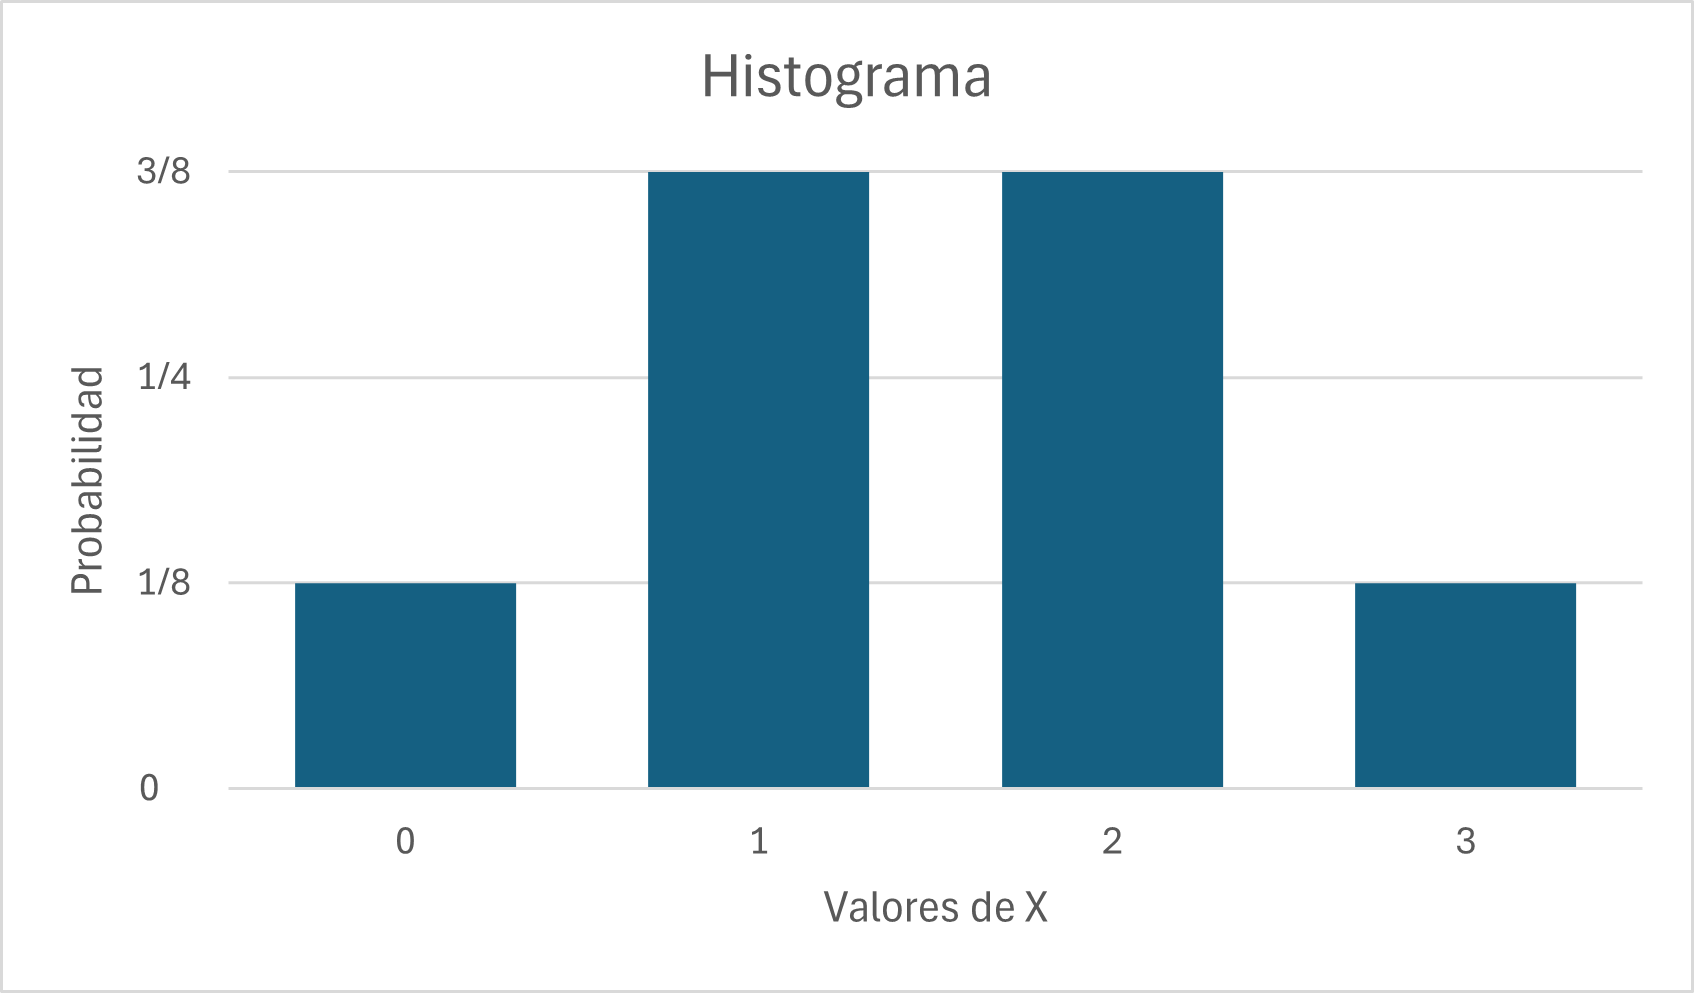
\includegraphics[width=0.8\textwidth]{./Assets/HistogramaT5P2.png}
    \end{figure}
\end{enumerate}



% ---------- Tarea 6 ----------
\newpage
\begin{center}
    { \LARGE Tarea 6}
\end{center}

\begin{enumerate}
    %  - Problema 1
    \item Un dado equilibrado se lanza dos veces consecutivas. Sea $X$ la diferencia entre el resultado del primer y el segundo lanzamiento.
    % Respuestas:
    \vspace{\Aspace} \par
    • Encuentre la función de probabilidad de $X$.
    \\ { \color{azul} $f(x) = P[X = x] = \frac{6 - |x|}{36}$ }

    \vspace{\Aspace} \par
    • Encuentre la función de distribución de $X$.
    \\ { \color{azul} $F(x) = \sum\limits_{x = -5}^{5} \frac{6 - |x|}{36}$ }

    \vspace{\Aspace} \par
    • Determinar el valor esperado de $X$.
    \\ { \color{azul} $E[X] = \mu = \sum\limits_{x = -5}^{5} x\frac{6 - |x|}{36} = 0$ }

    \vspace{\Aspace} \par
    • Determinar la varianza de $X$.
    \\ { \color{azul} $Var(X) = \sigma^{2} = \sum\limits_{x = -5}^{5} (x - \mu)^{2} (\frac{6 - |x|}{36}) = \frac{35}{6}$ }

    \vspace{\Aspace} \par
    • Determinar el histograma.
    \begin{figure}[h]
        \centering
        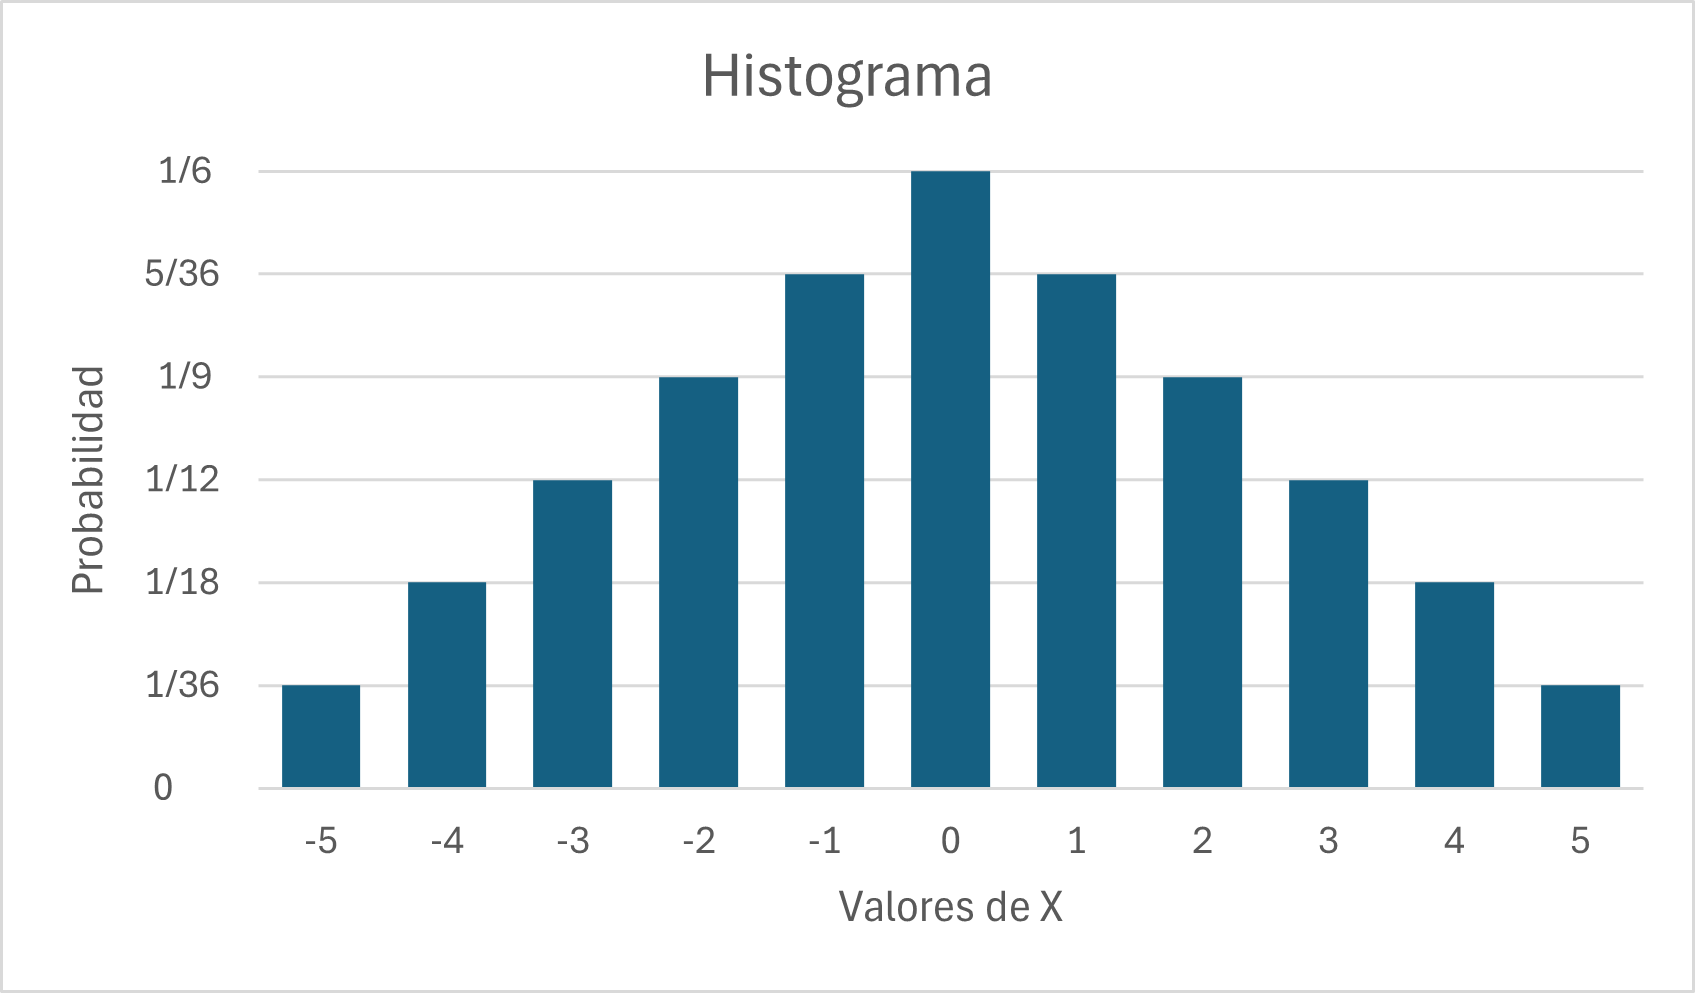
\includegraphics[width=0.6\textwidth]{./Assets/HistogramaT6P1.png}
    \end{figure}

    • Dibujar el valor esperado y el intervalo que resulta de estar dentro de una desviación estándar de la media.
    \vspace{\Aspace}
    \\ { \color{azul} $\sigma = \sqrt{\frac{35}{6}}$ }
    \begin{figure}[h]
        \centering
        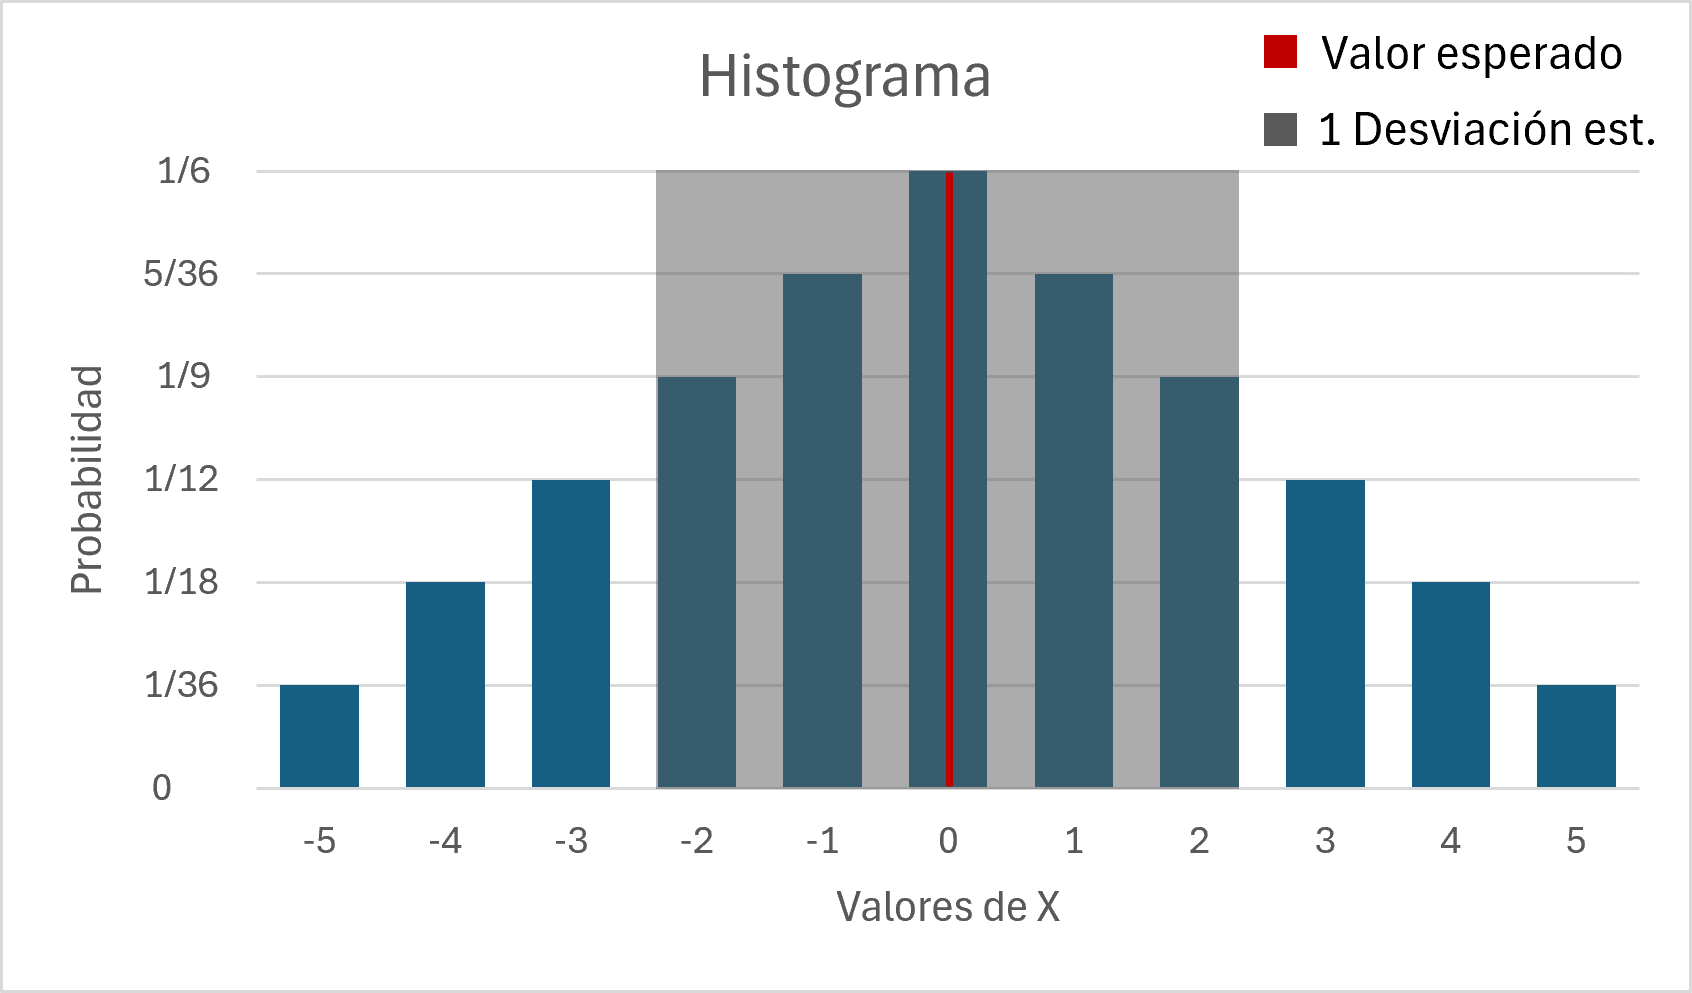
\includegraphics[width=0.6\textwidth]{./Assets/Histograma2T6P1.png}
    \end{figure}

    \newpage
    % - Problema 2
    \vspace{\Pspace}
    \item Se sabe que un jugador tiene una probabilidad del 95\% de ganar un juego importante. Sea $X$ la variable aleatoria que indica si gana o pierde el juego.
    % Respuestas:
    \vspace{\Aspace} \par
    a) ¿Sigue una distribución de Bernoulli?
    \\ { \color{azul} Dado que solo existen dos posibles resultados (éxito o fracaso), esta sigue una distribución de Bernoulli $X \sim Be(0{.}95)$ }

    \vspace{\Aspace} \par
    b) Si puediera jugar muchas veces el juego importante, ¿qué porcentaje de victorias esperaría observar?
    \\ { \color{azul} Si cada juego es independiente, $E[X] = 0{.}95 = 95\%$ }

    \vspace{\Aspace} \par
    c) ¿Cuál es la varianza de esta variable aleatoria?
    \\ { \color{azul} $Var(X) = \sigma^2 = 0{.}95 (1 - 0{.}95) = 0{.}0475$ }

    \vspace{\Aspace} \par
    d) Determine el intervalo de valores que están dentro de una desviación estándar de la media.
    \\ { \color{azul}
        $\sigma = \sqrt{0.0475} = \frac{\sqrt{19}}{20} = 0{.}218$ \vspace{0.1cm}
        \newline $[E[X]] - \sigma, E[X] + \sigma] = [0{.}95 - 0{.}218, 0{.}95 + 0{.}218] = [0{.}732, 1{.}168]$ \vspace{0.1cm}
        \newline Dado que no pueden haber valores mayores que 1, el intervalo termina siendo $[0{.}732, 1]$
    }
\end{enumerate}



% ---------- Tarea 7 ----------
\newpage
\begin{center}
    { \LARGE Tarea 7}
\end{center}

\begin{enumerate}
    %  - Problema 1
    \item Antes de la venta de pianos, deben probarse para saber si se encuentran en buen estado o defectuoso. El porcentaje de defectuosos es de 5\%. Sea $X$ el número de pianos en buen estado en una muestra aleatoria de tamaño $n = 25$,
    % Respuestas:
    \vspace{\Aspace} \par
    • ¿Qué tipo de distribución tiene $X$?
    \\ { \color{azul} Dado que solo existen dos posibles resultados (buen estado o defectuoso) y contamos con una muestra, esta sigue una distribución binomial $X \sim Bin(25, 0{.}95)$ }

    \vspace{\Aspace} \par
    • Determinar la probabilidad de observar exactamente 7 pianos en buen estado.
    \\ { \color{azul} $P[X = 7] = \binom{25}{7} (0{.}95)^{7} (0{.}05)^{18} = 1{.}28$x$10^{-18}$ }

    \vspace{\Aspace} \par
    • Determinar la probabilidad de observar 22 o más pianos en buen estado.
    \\ { \color{azul} $P[X \geq 22] = \sum\limits_{x = 22}^{25} \binom{25}{x} (0{.}95)^{x} (0{.}05)^{25 - x} = 0{.}966$ }

    \vspace{\Aspace} \par
    • Determinar la probabilidad de observar menos de 22 pianos en buen estado
    \\ { \color{azul} $P[X < 22] = 1 - P[X \geq 22] = 1 - 0{.}966 = 0{.}034$ }

    \vspace{\Aspace} \par
    • Determinar el número de pianos que espera encontrar en buen estado.
    \\ { \color{azul} $E[X] = (25)(0{.}95) = 23{.}75$ }

    \vspace{\Aspace} \par
    • Determinar la varianza de $X$.
    \\ { \color{azul} $Var(X) = \sigma^{2} = (25)(0{.}95)(0{.}05) = 1{.}1875$ }


    % - Problema 2
    \vspace{\Pspace}
    \item Una pareja desea tener una niña en su familia. La pareja decide tener hijos hasta que se tenga la primer niña. Suponga que la probabilidad de tener una hija es de 0.25. 
    % Respuestas:
    \vspace{\Aspace} \par
    • ¿Cuál es la probabilidad de que la familia tenga $x$ niñas?
    \\ { \color{azul}  }

    \vspace{\Aspace} \par
    • ¿Cuál es la probabilidad de que la familia tenga cuatro hijos?
    \\ { \color{azul}  }

    \vspace{\Aspace} \par
    • ¿Cuál es la probabilidad de que la familia tenga cuando mucho cuatro hijos?
    \\ { \color{azul}  }

    \vspace{\Aspace} \par
    • ¿Cuántos hijos esperaría que tenga esta familia?
    \\ { \color{azul}  }

    \vspace{\Aspace} \par
    • ¿Cuál es la desviación estándar?
    \\ { \color{azul}  }


    % - Problema 3
    \vspace{\Pspace}
    \item Sea $X$ una variable aleatoria tal que $ X \sim U\{1, 2, \dots, n\} $. Demuestre que:
    % Respuestas:
    \vspace{\Aspace} \par
    • $E(X^{2}) = \frac{(n + 1)(2n + 1)}{6}$
    \\ { \color{azul}  }

    \vspace{\Aspace} \par
    • $Var(X) = \frac{n^{2} - 1}{12}$ 
    \\ { \color{azul}  }
\end{enumerate}



% ---------- Tarea 8 ----------
\newpage
\begin{center}
    { \LARGE Tarea 8}
\end{center}

\begin{enumerate}
    %  - Problema 1
    \item Se sabe que, en promedio, llegan 15 personas por hora a una tienda departamental.
    \\ Conteste lo siguiente:
    % Respuestas:
    \vspace{\Aspace} \par
    • ¿Qué tipo de distribución tiene $X$?
    \\ { \color{azul}  }

    \vspace{\Aspace} \par
    • Determine la probabilidad de observar exactamente 15 personas en una hora.
    \\ { \color{azul}  }

    \vspace{\Aspace} \par
    • Determine la probabilidad de observar 5 o más personas en una hora.
    \\ { \color{azul}  }

    \vspace{\Aspace} \par
    • Determine la probabilidad de observar menos de 5 personas en una hora.
    \\ { \color{azul}  }

    \vspace{\Aspace} \par
    • Determine en número de personas que se espera que lleguen en una hora.
    \\ { \color{azul}  }

    \vspace{\Aspace} \par
    • Determinar la varianza de $X$.
    \\ { \color{azul}  }



    % - Problema 2
    \item Sean $X_{1} \sim Bin(n_{1}, p)$ y $X_{2} \sim Bin(n_{2}, p)$, dos variables aleatorias independientes con la misma probabilidad de éxito $p$.  
    Sea la variable aleatoria $Z = X_{1} + X_{2}$. Demuestra que $Z \sim Bin(n_{1} + n_{2}, p)$.  
    Recuerde que la función de probabilidad de $Z$ está dada por:
    \[
        P(Z = z) = \sum_{k = 0}^{z} P(X_{1} = k) P(X_{2} = z - k)
    \]
    \textbf{Hint}: Usa el siguiente resultado:
    \[
        \sum_{k = 0}^{z} \binom{n_{1}}{k} \binom{n_{2}}{z - k} = \binom{n_{1} + n_{2}}{z}
    \]
    % Respuesta:
    \vspace{\Aspace} \par
    { \color{azul}  }


    % - Problema 3
    \vspace{\Pspace}
    \item Genere números aleatorios de una variable aleatoria geométrica con parámetro 0.7 en cualquier lenguaje de programación. Para ello, siga estos pasos:
    \vspace{0.2cm}
    \\ • Genere un número aleatorio a partir de una distribución uniforme en $(0, 1)$.
    \\ • Utilice el criterio visto en clase basado en la inversa de la función de distribución acumulada de la variable geométrica para determinar el valor generado.
    % Respuesta:
    \vspace{\Aspace} \par
    { \color{azul}  }
\end{enumerate}

\end{document}
